\documentclass[../main]{subfiles}
\begin{document}
\chapter{枝の増減に伴う同期状態の変化}
\label{chap:method-3body}
\section{問題設定及び数値実験}
\label{sec:method-3body-settting}
ERモデル (Erd\H{o}s–R\'{e}nyi model) $\Gamma_{n,m}$ において,枝の本数$m$を変化することでモデルの構造を変化させることを振動子ネットワークで考える.
すなわち,$n$ 体の振動子ネットワークにおいて$m=0$から$m=n(n-1)/2$まで枝の本数を連続的に変化させる.
このとき,構造の変化に伴い同期状態が変化することが考えられる.\\
固有振動数の分布として,一般にはローレンツ分布などの連続分布\cite{kuramoto1975}から二項分布のような離散分布\cite{1992BonillaNeuSpigler}まで考えられる.
本論文では,異なる固有振動数を持つ振動子の同期を扱う最も簡単な分布としてニ項分布を用いる.
特に,一般性を失わず$\pm 1$の二項分布$\operatorname{Bin}(n,p)$を用いる.\\
$n=6$での数値実験の結果を図\ref{fig:cutting_N6K1}に示す.
ただし,時刻$t\ (0\leq t\leq T)$で位相$\phi_i(t)$の node $i$の実効振動数は,$\Omega_i^{\mathrm{eff}}:=(\phi_i(T)-\phi_i(T/2))/(T/2)$で定めた.\\
ここで,$m=2$における node $0,1$,$m=7$における node $0$のように,枝の増加により増加前に同期していた node と非同期になり別の node と同期する,つまり同期クラスタが変化する現象が見られる.
以下,このような同期状態の変化を「鞍替え」と呼ぶこととする.
この鞍替え現象は鎖構造の蔵本モデルにおいて結合強度を全て同じ値で変化させた場合に発生することが知られている\cite{XiaHuang:130506}ものの(付録参照),ネットワーク構造の変化で発生することは知られておらず,
疎なネットワークにおける微視的なクラスタリングパターンの理解において重要な役割を果たすと考えられる.
また,ネットワーク全体のクラスタリングパターンの変化は,一部の振動子についての同期現象と鞍替え現象に分割して理解することができる.\\
次節ではこの鞍替え現象に注目し解析を行う.
\begin{figure}[t]
\centering
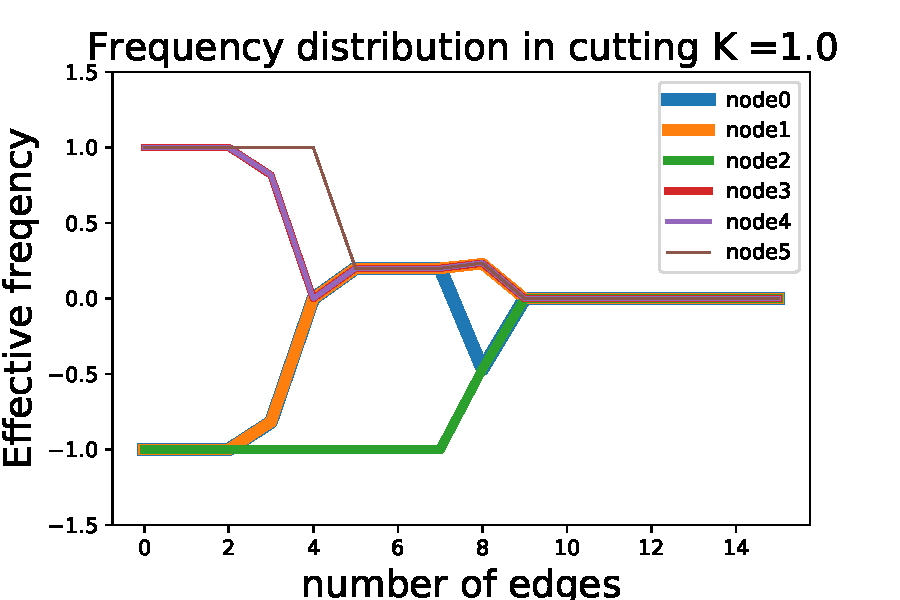
\includegraphics[width=105mm]{./images/cutting_N6K1.pdf}
\centering
\caption{固有振動数$1$の振動子3つと固有振動数の$-1$の振動子3つからなる6体の振動子ネットワークにおいて,枝を1本ずつランダムに選び全接続まで連続的に増やしたときの各振動子の実効振動数の変化を表す.
$m=2$におけるnode $0,1$,$m=7$におけるnode $0$では,枝の増加により増加前に同期していたnodeと非同期になり別のnodeと同期する「鞍替え」が見られる.}
\label{fig:cutting_N6K1}
\end{figure}
\section{鞍替え現象のモデル化}
ある1つの振動子が$M$体の集団から$N$体の別の集団に鞍替えを起こすとき,以下のようにモデル化できる.
\begin{screen}
固有振動数$\omega$の振動子が実効振動数$\omega_M$の$M$体の振動子集団$\Omega_M$との間に$m$本の枝で繋がっており,また,実効振動数$\omega_N$の$N$体の振動子集団$\Omega_N$との間に$n$本の枝で繋がっている.
ただし,振動子集団$\Omega_M$と振動子集団$\Omega_N$との間に枝は存在しないとする.(図\ref{fig:switch})\\
枝の本数$m,n$が変化すると,振動子の実効振動数が変化し鞍替えが生じる.
\end{screen}
\begin{figure}[t]
\centering
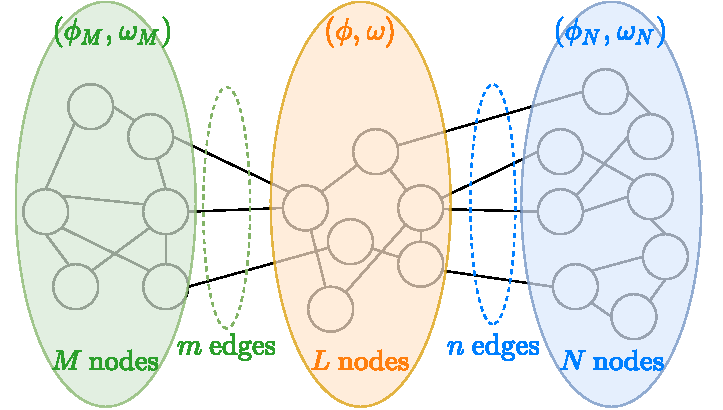
\includegraphics[width=105mm]{./images/three_obj_before.pdf}
\centering
\caption{鞍替え現象に関わる部分ネットワーク}
\label{fig:switch}
\end{figure}
このとき,それぞれの振動子集団に属する振動子がそれぞれ同一の位相・固有振動数を持つとして平均場近似を行うと,発展方程式は以下のようになる.
\begin{align*}
    \dot{\phi}&=\omega+mK\sin\left( \phi_N-\phi \right)+nK\sin\left( \phi_M-\phi \right)\\
    \dot{\phi}_M&=\omega_M+\frac{m}{M}K\sin\left( \phi-\phi_M \right) \\
    \dot{\phi}_N&=\omega_N+\frac{n}{N}K\sin\left( \phi-\phi_N \right)    
\end{align*}
ここで,結合強度比$a=n/m,\ N=1,\ M=1$と仮定すると,図\ref{fig:3body}のような鞍替えする振動子を中央とする鎖状の3体ネットワークに簡略化される.\\
\begin{figure}[t]
    \centering
    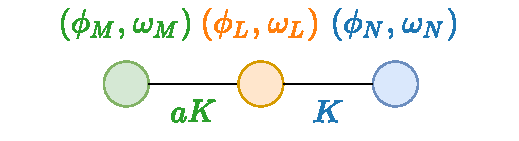
\includegraphics[width=105mm]{./images/three_obj_after.pdf}
    \centering
    \caption{鞍替え現象に関わる部分ネットワークを簡略化した鎖状の3体ネットワーク}
    \label{fig:3body}
\end{figure}
\begin{align}
    \label{eq:3body}
    \begin{split}
        \dot{\phi}&=\omega+K\sin\left( \phi_N-\phi \right)+aK\sin\left( \phi_M-\phi \right)\\
        \dot{\phi}_M&=\omega_M+aK\sin\left( \phi-\phi_M \right) \\
        \dot{\phi}_N&=\omega_N+K\sin\left( \phi-\phi_N \right)    
    \end{split}
\end{align}
3体系においてパラメータを変化させることで2体の同期に関わる鞍替え現象を観測できることが予想されると同時に,3体全体の同期現象を調べることもできる.
ネットワーク全体の同期状態の変化は部分ネットワークそれぞれの同期状態の変化で理解されるため,
簡略化した3体系の同期状態を調べることでネットワーク全体の同期状態の変化を理解することに繋がると期待される.\\
次節では,3体系について鞍替え現象より広い範囲での同期状態を調べる.
\section{3体系の同期状態}
元の部分ネットワーク (図\ref{fig:switch}) における枝の数$m,\ n$の変化は,3体系 (図\ref{fig:3body}) においてはパラメータ$a,\ K$の変化に対応する.

3体系について,様々な振動数差$\Omega,\ \omega$に対し,結合強度比$a$を様々な値で固定し結合強度$K$を変化させると,同期状態の変化が図\ref{fig:3body-abs}の4パターン見られた.
\begin{figure}[t]
    \begin{minipage}[b]{0.47\linewidth}
      \centering
      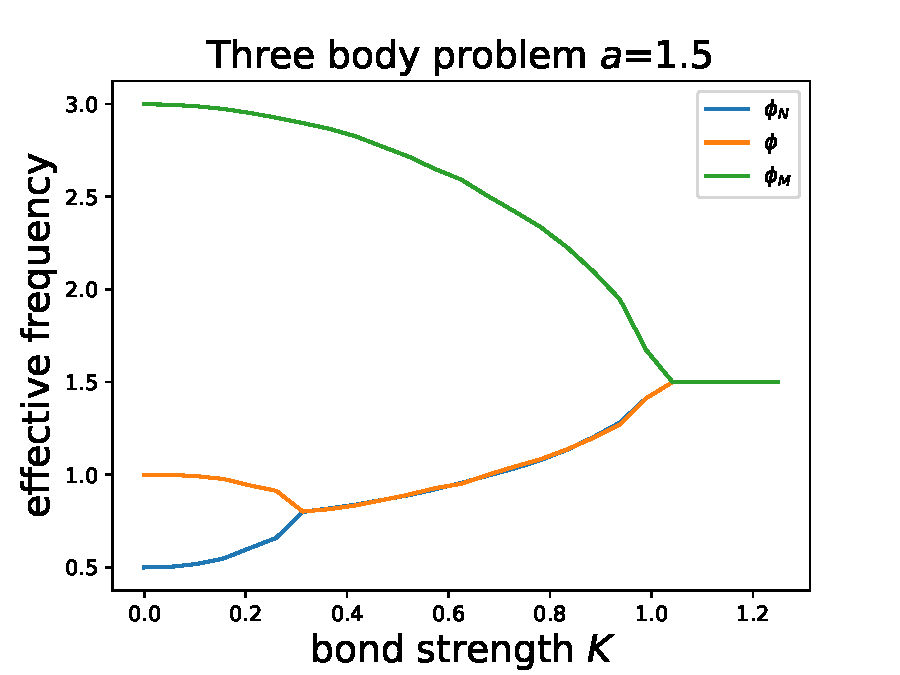
\includegraphics[keepaspectratio, scale=0.42]{images/three-body-prob-notapprox-a150.pdf}
      \subcaption[c]{$a=1.5,\ \Omega=-2,\ \omega=0.5$.\\3種類の同期状態を経ている.}
      \label{fig:3body-notapprox150}
    \end{minipage}
    \begin{minipage}[b]{0.47\linewidth}
      \centering
      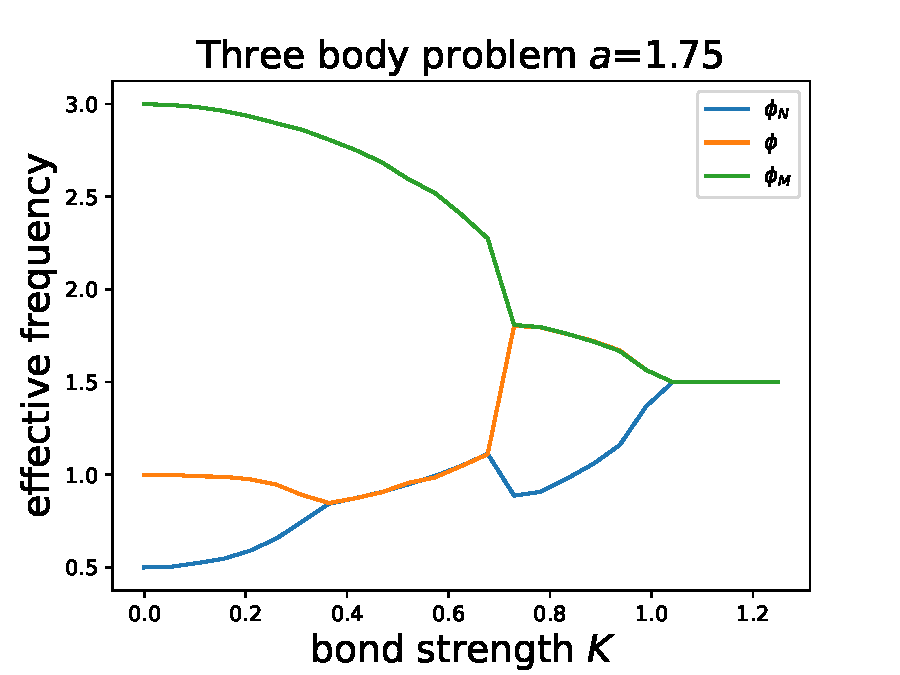
\includegraphics[keepaspectratio, scale=0.42]{images/three-body-prob-notapprox-a175.pdf}
      \subcaption{$a=1.75,\ \Omega=-2,\ \omega=0.5$.\\5種類の同期状態を経ている.}
      \label{fig:3body-notapprox175}
    \end{minipage}\\
    \begin{minipage}[b]{0.47\linewidth}
      \centering
      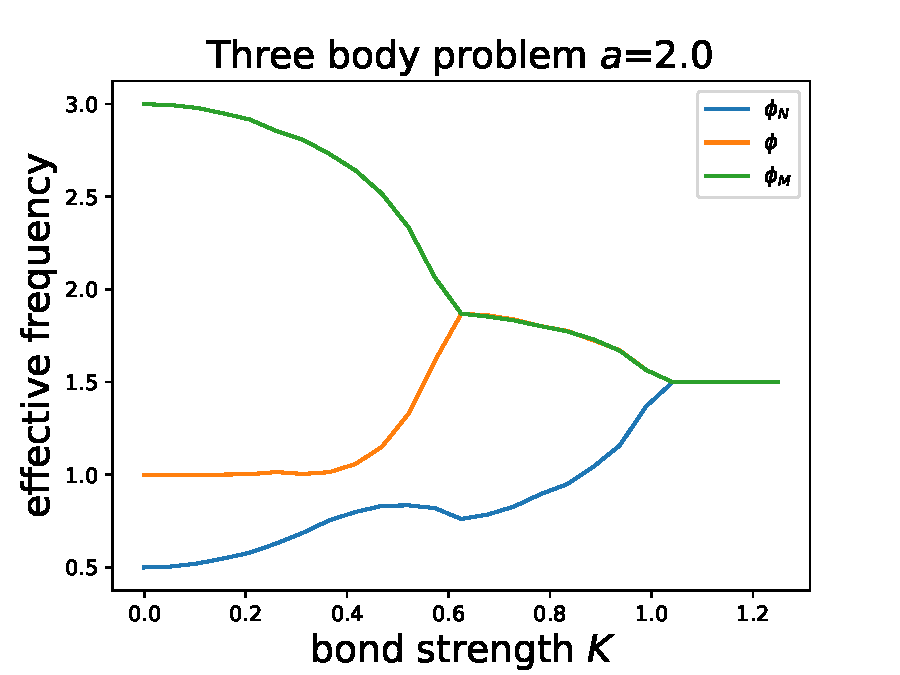
\includegraphics[keepaspectratio, scale=0.42]{images/three-body-prob-notapprox-a200.pdf}
      \subcaption{$a=2.0,\ \Omega=-2,\ \omega=0.5$.\\3種類の同期状態を経ている.}
      \label{fig:3body-notapprox200}
    \end{minipage}
    \begin{minipage}[b]{0.47\linewidth}
      \centering
      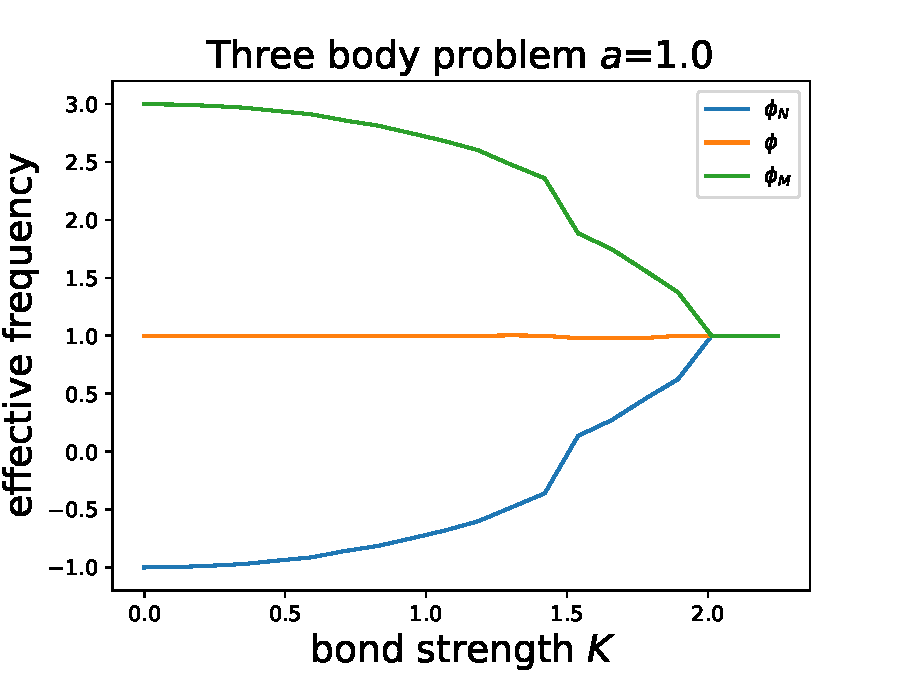
\includegraphics[keepaspectratio, scale=0.42]{images/three-body-prob-symmetry-a100.pdf}
      \subcaption{$a=1.0,\ \Omega=-2,\ \omega=2$.\\2種類の同期状態を経ている.}
      \label{fig:3body-symmetry}
    \end{minipage}
    \caption{様々なパラメータ$a,\ \Omega,\ \omega$で結合強度$K$を変化させたときの同期状態の変化}
    \label{fig:3body-abs}
\end{figure}
最大で5つの同期状態が存在し,4つの臨界結合強度が存在することがわかった.
どのパターンの臨界結合強度も,図\ref{fig:3body-notapprox175}のパターンにおける臨界結合強度の一部が存在する場合として考えることができる.
つまり,図\ref{fig:3body-notapprox150}は$K=0.7$付近の臨界結合強度が2つとも存在せず$K=0.3,\ K=1.0$付近の臨界結合強度が存在する場合として解釈できる.
図\ref{fig:3body-notapprox175}は$K=0.7$付近の臨界結合強度が1つだけ存在し$K=1.0$付近の臨界結合強度が存在する場合として解釈できる.
そして,図\ref{fig:3body-symmetry}は一番大きい臨界結合強度だけが存在する場合として解釈できる.\\
よって,3体系のふるまいを理解する上では,図\ref{fig:3body-notapprox175}の場合の同期状態の変化及び臨界結合強度を解析するだけで十分である.

特に,次節以降の解析の都合,図\ref{fig:3body-notapprox175}と同様に最も多様に同期状態が変化するパラメータであり,
$|\Omega|\gg|\omega|$となる$a=4.0,\ \Omega=-2,\ \omega=0.1$の場合について注目する.
そのときの結合強度と実効振動数の関係を図\ref{fig:3body-state}に示す.
\begin{figure}[t]
\centering
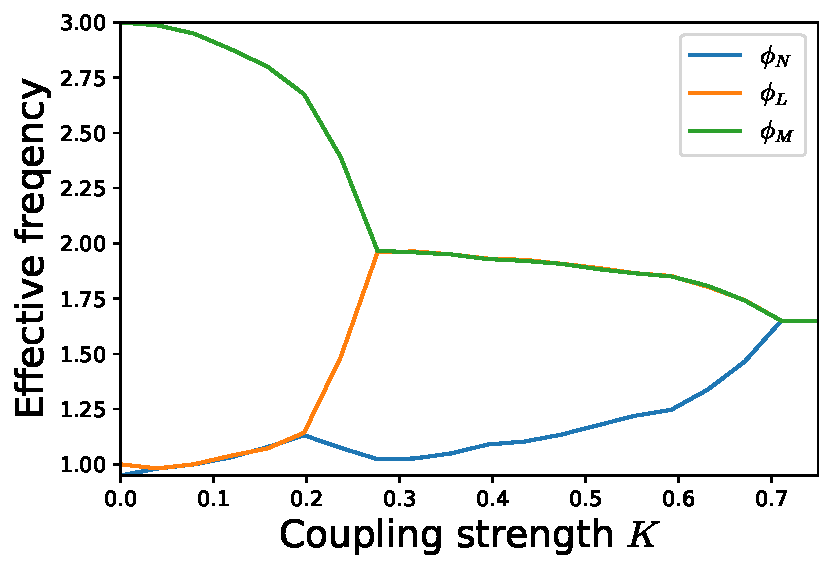
\includegraphics[width=105mm]{./images/three-body-prob.pdf}
\centering
\caption{3体ネットワークで$a=4.0,\ \Omega=-2,\ \omega=0.1$のしたときの結合強度$K$と実効振動数の関係.$0\leq K\lesssim 0.05$では3体が非同期であり (phase 1),$0.05\lesssim K\lesssim 0.15$では固有振動数の近い2体が同期する($\phi=\phi_N$, phase 2).そして,$0.15 \lesssim K\lesssim 0.27$では鞍替えが起こり非同期になり (phase 3),$0.27\lesssim K\lesssim 0.7$では振動数の遠い2体が同期する ($\phi=\phi_N$,\ phase 4).最後に$K\gtrsim 0.7$では3体が同期する (phase 5).}
\label{fig:3body-state}
\end{figure}
4つの臨界結合強度を分岐点として5つの同期状態に分岐することが分かる.
そこで,4つの臨界結合強度を小さい順にそれぞれ$K_1,\ K_2,\ K_3,\ K_4$とする.
すると,次のようにまとめられる.\\
$0\leq K<K_1$では3体が非同期であり (phase 1),$K_1\leq K<K_2$では固有振動数の近い2体が同期する ($\phi=\phi_N$,\ phase 2).そして,$K_2\leq K<K_3$では鞍替えが起こり非同期になり (phase 3),$K_3\leq K<K_4$では振動数の遠い2体が同期する($\phi=\phi_N$,\ phase 4).最後に$K\leq K_4$では3体が同期する (phase 5).\\
次節ではこれらの5つの同期状態が相平面上でどのように記述されるかを調べる.
\section{3体系の同期状態の相平面解析}
$x=\phi_M-\phi,\ y=\phi_N-\phi$と位相差を取ると,式\eqref{eq:3body}は2本の位相差方程式になる.
\begin{align}
    \label{eq:phase-diff}
    \begin{split}
    \dot{x}&=\Omega-K(2a\sin x+\sin y)\\
    \dot{y}&=\omega-K(a\sin x+2\sin y)
    \end{split}
\end{align}
図\ref{fig:3body-state}のそれぞれの同期状態に対応する$x-y$平面上の相図を図\ref{fig:phase}に示す.

\captionsetup[figure]{justification=centering}
\begin{figure}[t]
    \begin{minipage}[b]{0.47\linewidth}
      \centering
      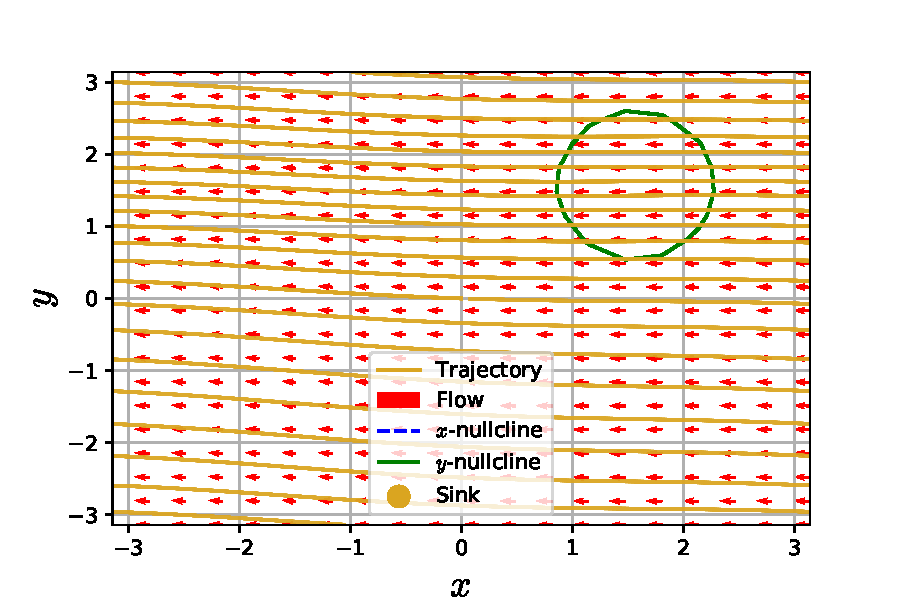
\includegraphics[keepaspectratio, scale=0.42]{images/phase_a4K2.pdf}
      \subcaption{$K=0.02$.3体が非同期.\\phase 1}
      \label{fig:phase-k2}
    \end{minipage}
    \begin{minipage}[b]{0.47\linewidth}
      \centering
      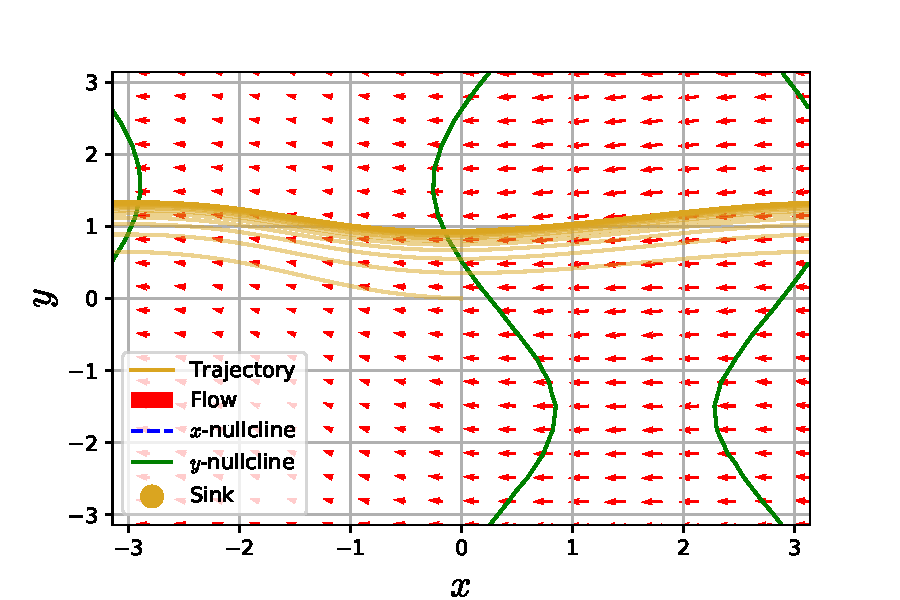
\includegraphics[keepaspectratio, scale=0.42]{images/phase_a4K10.pdf}
      \subcaption[c]{$K=0.1$.固有振動数が近いものと同期.\\phase 2}
      \label{fig:phase-k10}
    \end{minipage}\\
    \begin{minipage}[b]{0.47\linewidth}
      \centering
      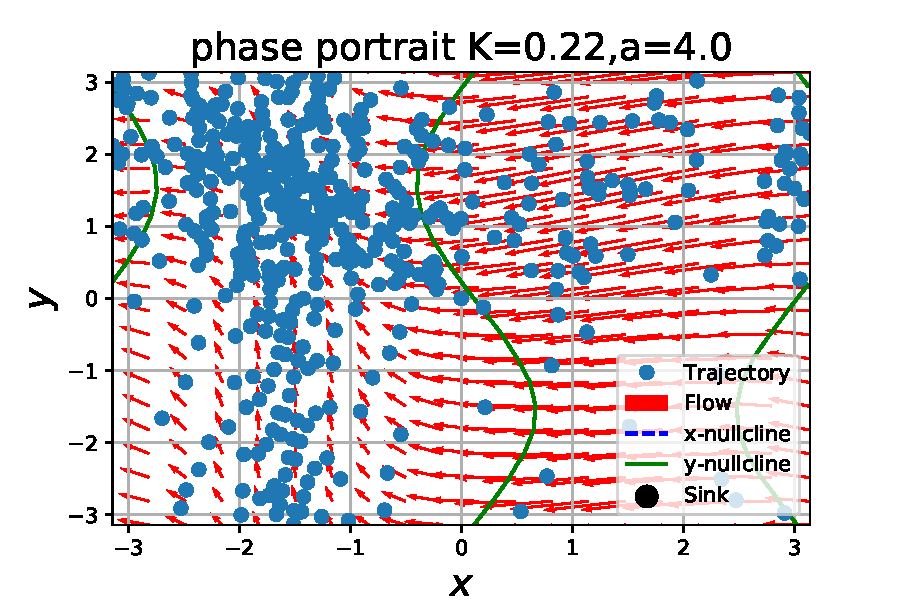
\includegraphics[keepaspectratio, scale=0.42]{images/phase_a4K22.pdf}
      \subcaption{$K=0.22$.鞍替え後3体が非同期.\\phase 3}
      \label{fig:phase-k22}
    \end{minipage}
    \begin{minipage}[b]{0.47\linewidth}
      \centering
      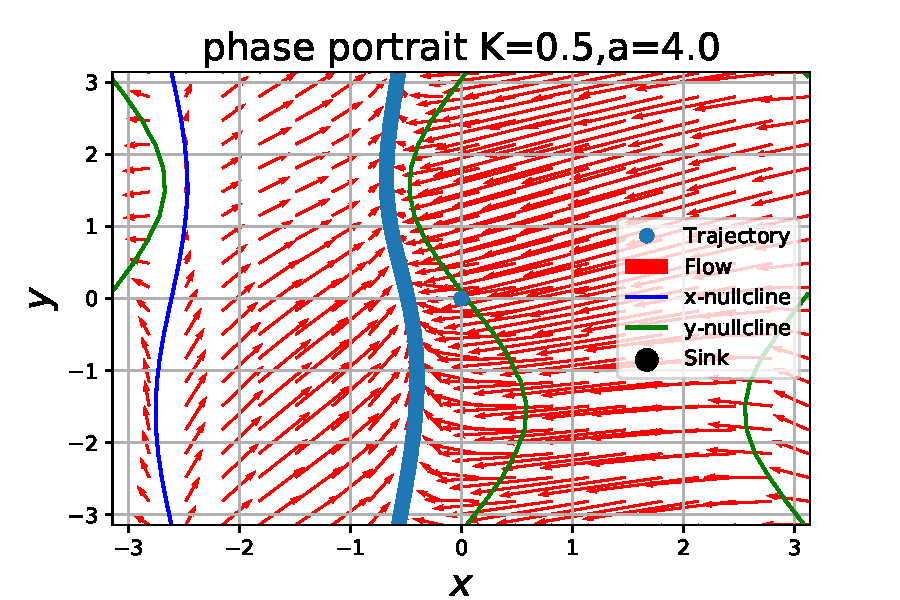
\includegraphics[keepaspectratio, scale=0.42]{images/phase_a4K50.pdf}
      \subcaption{$K=0.5$.固有振動数が遠いものと同期.\\phase 4}
      \label{fig:phase-k50}
    \end{minipage}\\
    \begin{minipage}[b]{0.47\linewidth}
      \centering
      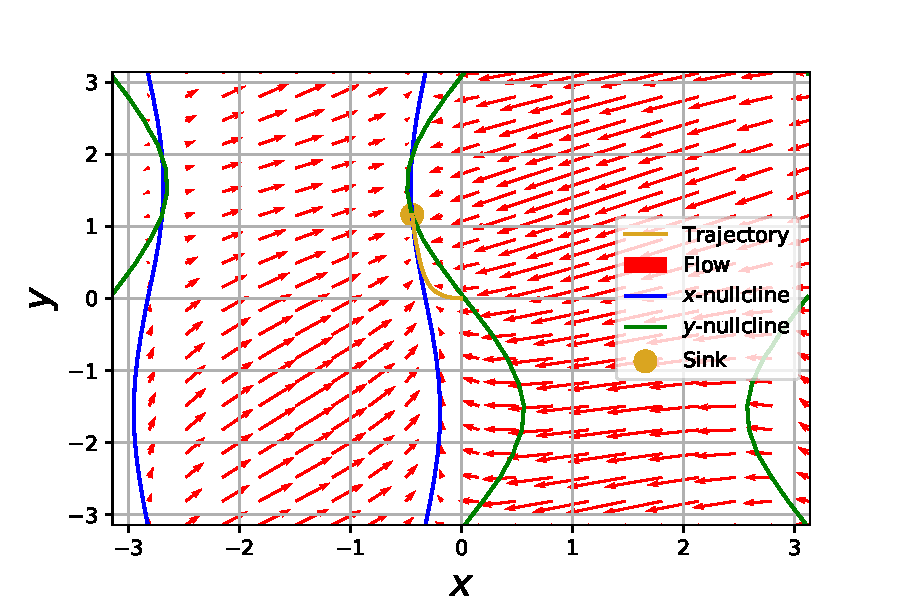
\includegraphics[keepaspectratio, scale=0.42]{images/phase_a4K80.pdf}
      \subcaption{$K=0.8$.3体とも同期.\\phase 5}
      \label{fig:phase-k80}
    \end{minipage}
    \caption{$a=4.0,\ \omega=0.1,\ \Omega=2$における5つの同期状態における相図.\\
    ベクトル場,$x,\ y$-nullcline,沈点,及び$(x,y)=(0,0)$から発する軌道を示している.}\label{fig:phase}
\end{figure}
\clearcaptionsetup{figure}

それぞれの同期状態は2本の位相差方程式の安定解に対応し,それぞれ以下のような現象に対応する.
\begin{itemize}
    \item 
    2振動子の同期:任意の初期位相差から位相差$x,y$の片方のみが安定な$\mathbb{S}^1$と同相な周期軌道へ収束する.(図\ref{fig:phase-k10},\ \ref{fig:phase-k50})
    \item
    3振動子の同期:任意の初期位相差から位相差$x,y$の両方とも安定な平衡点へ収束する.(図\ref{fig:phase-k80})
    \item
    非同期:ほとんど確実に,安定な周期軌道が存在せず,$\mathbb{T}^2$全てを覆うような準周期軌道を描く.(図\ref{fig:phase-k2},\ \ref{fig:phase-k22})
\end{itemize}
以上の相平面解析の結果を元に,以降の節では4つ臨界結合強度を求める.
\section{臨界結合強度の近似解}
\label{sec:3body-critical}
    \subsection{固有振動数の近い2体との同期 ($K_1$,$K_2$)}
    \label{sec:3body-k12}
    本節では解析のために2つの振動数差が大きく異なるとし,以下の関係を仮定する.
    \begin{align}
        \label{eq:assume}
        |\Omega|\gg|\omega|
    \end{align}
    固有振動数差$\Omega,\ \omega$に比べ,結合強度$K$が小さい状況($K\leq K_1$)では,以下の大小関係が成り立つ.
    \begin{align}
        \label{eq:k1-approx}
        |\Omega|\gg|\omega|>K
    \end{align}
    また,
    結合強度$K$が固有振動数差$\Omega$に比べ小さく,固有振動数差$\omega$に比べ大きい状況($K\sim K_2$)では,以下の大小関係が成り立つ.
    \begin{align}
        \label{eq:k2-approx}
        |\Omega|\gg K>|\omega|
    \end{align}
    式\eqref{eq:k1-approx},\ \eqref{eq:k2-approx}両方の状況とも,平均的に$x$は固有振動数$\Omega$で変化し,$y$は$\omega\ (|\omega|\ll|\Omega|)$で変化する.
    よって,タイムスケールの分離を行うことができる.
    つまり,$\dot{x}=\Omega,\ y=z\ (\dot{z}=\omega)$に対して,$K$に依存した周期外力が摂動した系として近似できる.\\
    式\eqref{eq:phase-diff}において,$\tau:=\Omega t,\ \varepsilon:=\omega/\Omega,\ k=K/\Omega,\ S(x,y)=-a\sin x-2\sin y$とすると,位相差$y$の時間発展は以下のように表される.
    \begin{align*}
        \dv{y}{\tau}=\varepsilon+k S(x,y) 
    \end{align*}
    このとき,$y$を以下のように近恒等変換する.
    \begin{align}
        y=z+kh_1(z,\tau)+k^2h_2(z,\tau)+O(k^3)
        \label{eq:pertu-ytilde}
    \end{align}
    ここで,$h_i$は$i=1,2,\ h_i(z+2\pi,\tau+2\pi)=h_i(z,\tau),h_i(z,0)=0$を満たす関数とする.\\
    一方$x$については$k$の1次で展開すると,
    \begin{align*}
        x&=\Omega t-\Omega k\int_0^t(2a\sin \Omega s+\sin z)\dd{s}+O(k^2)\\ 
        &=\tau+\Omega k\left(\frac{2a}{\Omega}\cos\tau+\frac{\tau}{\Omega}\sin z\right)+O(k^2)
    \end{align*}
    最終行では,$\cos x(0)=0,\ \cos y(0)=0$となるように初期時刻$t=0$を定めたことに因る.\\
    また,$S(x,y)$を$z,\ t$に関して展開する.
    \begin{align*}
        S(x,y)&=-a\sin x-2\sin y\\
        &=-a\sin\tau-2\sin z-2 kh_1\cos z\\
        &-a\cos\tau\cdot \Omega k\left(\frac{2a}{\Omega}\cos \tau+\frac{\tau}{\Omega}\sin z\right)+O(k^2)\\
        &=-a\sin\tau-2\sin z+k\left(-2 \cos z\cdot h_1-2a^2\cos^2\tau-a\tau\cos \tau\sin z\right)\\
        &+O(k^2)
    \end{align*}
    さらに,$S_1:=-a\sin\tau-2\sin z,\ S_2:=-2a^2\cos^2\tau-a\tau\cos \tau\sin z$と定めると,
    \begin{align*}
        S(x,y)=S_1+k\pt_y S_1\cdot h_1+kS_2
    \end{align*}
    となる.\\
    式\eqref{eq:pertu-ytilde}を両辺$\tau$で微分すると,$\dot{\ast}=\dd{\ast}/\dd{\tau}$として,
    \begin{align*}
        \dv{y}{\tau}&=\dot{z}+k(\dot{z}\partial_zh_1+\partial_\tau h_1)+k^2(\dot{z}\partial_zh_2+\partial_\tau h_2)+O(k^3)\\
        &=(1+k\partial_zh_1+k^2\partial_zh_2)\dot{z}+k\pt_\tau h_1+k^2\pt_\tau h_2+O(k^3)
    \end{align*}
    整理すると,
    \begin{align*}
        \dot{z}&=(1+k\pt_zh_1+k^2\pt_zh_2)^{-1}\left( \dv{y}{t}-k\pt_\tau h_1-k^2\pt_\tau h_2 \right)+O(k^3)\\
        &=(1-k\pt_zh_1-k^2\pt_zh_2)\left(\varepsilon+kS_1+k^2 \pt_y S_1h_1+k^2S_2-k\pt_\tau h_1-k^2\pt_\tau h_2 \right)\\
        &=\varepsilon+k(S_1-\pt_\tau h_1-\varepsilon\pt_zh_1)\!+\!k^2\left(\pt_y S_1h_1 -\pt_\tau h_2-\varepsilon\pt_zh_2 -\pt_zh_1(S_1-\pt_\tau h_1)+S_2\right)
    \end{align*}
    $\dot{z}$が以下のように展開されるとする.
    \begin{align*}
        \dot{z}=\varepsilon+kH_1(z-\varepsilon \tau)+k^2H_2(z-\varepsilon \tau)+O(k^3)
    \end{align*}
    ここで,$z$が平均的に振動数$\omega$ (無次元時間$\tau$では$\varepsilon$) で変動することから$H_1,\ H_2$が$z-\varepsilon \tau$に依存するものとした.\\
    このとき,$k$の1次を比較すると新たな変数$s$を用いて以下の式が成立する.
    \begin{align*}
        H_1(z-\varepsilon \tau)=S_1(z+\varepsilon s,\tau+s)-\pt_s h_1(z+\varepsilon s,\tau+s)
    \end{align*}
    $s=0$から$s=-\tau$で両辺積分すると,
    \begin{align}
        -\tau H_1(z-\varepsilon \tau)&=\int_0^{-\tau}\left(-a\sin(\tau+s)-2\sin(z+\varepsilon s)\right)\dd{s}+h_1(z,\tau)\notag \\
        &=a \sin\tau+\frac{2}{\varepsilon}(\cos (z-\varepsilon t)-\cos  z)+h_1(z,\tau)\notag\\
        &=a \sin\tau+\frac{2}{\varepsilon}(\cos z+\varepsilon \tau\sin z-\varepsilon^2\tau^2/2\cdot\sin z-\cos z)+h_1(z,\tau)\notag\\
        &=a \sin\tau+2\tau\sin z-\varepsilon \tau^2\cos z+h_1(z,\tau)+O(\varepsilon^2)
        \label{eq-h1-H1}
    \end{align}
    $\tau=-2\pi$を代入して,
    \begin{align*}
        2\pi H_1\left(z+ 2\pi\varepsilon\right)&=-4\pi\sin z-4\pi^2\varepsilon \cos z+O(\varepsilon^2)\\
        H_1\left(z+2\pi\varepsilon\right)&=-2 \sin z-2\pi\varepsilon \cos z+O(\varepsilon^2)\\
        H_1\left(z+2\pi\varepsilon\right)&=H_1(z)+H_1'(z) 2\pi\varepsilon+O(\varepsilon^2)
    \end{align*}
    下2式を比較すると,
    \begin{align*}
        H_1(z)=-2\sin z+2\pi\varepsilon \cos z+O(\varepsilon^2)
    \end{align*}
    が得られる.
    式\eqref{eq-h1-H1}に代入すると,
    \begin{align*}
        h_1(z,\tau)&=2\tau\sin(z-\varepsilon \tau)-2\pi\varepsilon \tau\cos(z-\varepsilon \tau)-a\sin\tau-2\tau\sin z+\varepsilon \tau^2\cos z\\
        &=2\tau(\sin z-\varepsilon \tau\cos z-\sin z)-a\sin\tau+\varepsilon(-2\pi \tau+\tau^2)\cos z+O(\varepsilon^2)\\
        &=-a\sin\tau-\varepsilon(2\pi \tau+\tau^2)\cos z+O(\varepsilon^2)
    \end{align*}
    次に$\dot{z}$の$k$の2次を比較し,$h_1$を代入する.
    \begin{align*}
        H_2(z-\varepsilon \tau)=&\pt_y S_1h_1 -\pt_\tau h_2-\varepsilon\pt_zh_2 -\pt_zh_1(S_1-\pt_\tau h_1)+S_2\\
        =&-2\cos (z+\varepsilon s)\left( -a\sin(\tau+s)-\varepsilon(2\pi (\tau+s)+(\tau+s)^2) \cos (z+\varepsilon s) \right)-\pt_\tau h_2\\
        -&2a^2\cos^2(\tau+s)-a(\tau+s)\cos (\tau+s)\sin (z+\varepsilon s)+O(\varepsilon^2)\\
        +&\varepsilon(2\pi(\tau+s)+(\tau+s)^2)\sin (z+\varepsilon s) \\
        &\left( -a\sin(\tau+s)-2\sin (z+\varepsilon s) +a\cos(\tau+s)+\varepsilon(2\pi +2(\tau+s))\cos (z+\varepsilon s)\right)
    \end{align*}
    両辺$s=0$から$s=-\tau$で積分して,$\sin\tau\sim 0,\ \cos\tau\sim 1$とすると,
    \begin{align*}
        -\tau H_2(z-\varepsilon \tau)&=2a\cdot -\varepsilon \tau\sin z+4\pi\varepsilon\left( -\frac{\tau^2}{4} -\frac{\tau^2}{4}\cos 2z\right)+2\varepsilon\left( -\frac{\tau^3}{6} -\frac{\tau^3}{6}\cos 2 z\right)\\
        &-2\pi a\varepsilon\cdot\left(\tau\sin z\right)+2\pi a\varepsilon\left(-\varepsilon \tau\cos z\right)\\
        &-4\pi\varepsilon\left(-\frac{\tau^2}{4}+\frac{\tau^2}{4}\cos 2 z\right)-2\varepsilon\left( -\frac{\tau^3}{6} +\frac{\tau^3}{6}\cos 2z\right)+O(\varepsilon^2)\\
        &-a\varepsilon\left( \tau^2\sin z \right)+a\varepsilon\left( -2\tau^2\sin z \right)\\
        &-2a^2\left( -\frac{\tau}{2}-\frac{1}{4} \sin 2\tau\right)-a\left( -\tau \cos z\right)\\
        &=-2a\varepsilon \tau\sin z-2\pi\varepsilon\tau^2\cos 2 z-\frac{2}{3}\varepsilon\tau^3\cos 2z\\
        &-2\pi a\varepsilon \tau\sin z-3a\varepsilon\tau^2\sin z+a\tau(a+\cos z)+\frac{a^2}{2}\sin 2\tau
    \end{align*}
    $\tau=-2\pi$を代入して整理すると,
    \begin{align*}
        &H_2(z+2\pi\varepsilon )=-a(a+\cos z)\\
        +&2\varepsilon\left( a\sin z-2\pi^2\cos2 z+\frac{4\pi^2}{3} \cos 2 z+\pi a\sin z-3\pi a\sin z\right)
    \end{align*}
    以上で,位相差$y$の近恒等変換$z$の従う微分方程式を近似的に求めることができる.
    よって,$z$が安定解を持つ条件を求めることで$y$が安定解を持つ条件を求めることができる.\\
    まず,式\eqref{eq:k1-approx}の状況では,
    \begin{align*}
        \dot{z}&=\varepsilon-2k\sin z
    \end{align*}
    となる.これは,式\eqref{eq:phase-diff}に対し$x$の周期で平均化を行った($\sin x\sim 0$)式である.\\
    $z$が安定解を持つ条件は,
    \begin{align*}
        k\geq\frac{\varepsilon}{2}
    \end{align*}
    となり,臨界結合強度$K_1$は,
    \begin{align*}
        K_1=\frac{\omega}{2}
    \end{align*}
    となる.\\
    次に,式\eqref{eq:k2-approx}の状況を考える.
    閉形式で$K_2$を求めるため$|\varepsilon| \ll 1$を仮定すると,$H_2(z)=-a(a+\cos z)+O(\varepsilon)$となる.
    そして$k,\ \varepsilon$が十分小さいとして,$2$次以下の微小量を無視すると,$z$は以下のような微分方程式に従う.
    \begin{align*}
        \dot{z}&=\varepsilon-2k\sin z-k^2a(a+\cos  z)\\
        &=\varepsilon-a^2k^2-k\sqrt{4+a^2k^2}\sin ( z-\alpha)\quad(\alpha:\mathrm{const})
    \end{align*}
    $z$が安定解を持つ条件は,
    \begin{align*}
        |\varepsilon-a^2k^2|&\leq k\sqrt{4+(2\pi\varepsilon-ak)^2}\\
        0\leq |k|&\leq \sqrt{\frac{1}{a^4-a^2}\left(2+a^2\varepsilon+\sqrt{(2+2a^2\varepsilon)^2-\varepsilon^2(a^4-a^2)}\right)}
    \end{align*}
    となり,臨界結合強度$K_2$は,
    \begin{align*}
        K_2=|\Omega|\cdot\sqrt{\frac{1}{a^4-a^2}\left(2+a^2\varepsilon+\sqrt{(2+2a^2\varepsilon)^2-\varepsilon^2(a^4-a^2)}\right)}
    \end{align*}
    となる.    
    
    \subsection{固有振動数の遠い2体との同期($K_3$)}
    \label{sec:3body-k3}
    固有振動数の遠い2体との同期については,以下の命題\ref{prop:suff}により,
    \begin{align*}
        K_3\lessapprox \frac{|\Omega|}{2a-1}:=K'_3
    \end{align*}
    を得た.
    \begin{proposition}
        \label{prop:suff}
        トーラス$\mathbb{T}^2$上の自律系
        \begin{align}
            \label{eq:prop-2phase}
            \begin{split}
                \dot{x}&=\Omega-K(2a\sin x+\sin y)\\
                \dot{y}&=\omega-K(a\sin x+2\sin y)
            \end{split}
        \end{align}
        において,平衡点を持たず,任意の$y$に対し$\dot{x}=0$が解を持つならば,
        つまり,$K,a$が
        \begin{align*}
            K\geq \frac{|\Omega|}{2a-1}
        \end{align*}
        を満たすならば,
        2つの安定,不安定な$x$-$\mathrm{nullcline}$付近に$\mathbb{S}^1$と同相な安定,不安定な周期解がそれぞれ1つずつ存在し,任意の点から発する軌道は2つの周期解のどちらかに収束する.
    \end{proposition}
    まず,以下の補題を示す.
    \begin{lemma}
        \label{lemma:annulus}
        命題\ref{prop:suff}の状況で
        安定な$x$-nullclineの$x$座標の最大値・最小値をそれぞれ$x_{\max},\ x_{\min}$とし,$D=[x_{\min},x_{\max}]\times (-\pi,\pi ]\subset\mathbb{T}^2$とする.
        このとき,円筒領域$D$内に$\mathbb{S}^1$に同相な安定な周期解がただ一つ存在する.        
    \end{lemma}
    \begin{proof}
        まず,$D$内の任意の点から発する軌道は$D$内に留まる.
        なぜなら,$D$内の点から発して$D$外に出る軌道が存在すると仮定すると$D$の境界上で$D$外の流れを持つが,図\ref{fig:phase-k50}よりそのような点は存在しないからである.\\
        そして,命題\ref{prop:suff}の仮定より平衡点は存在せず,$D$は円環に同相でトーラス$\mathbb{T}^2$と同相でない.\\
        以上より,Poincar\'{e}-Bendixsonの定理の一般化 (定理\ref{thm:poiben-gen}) から$D$内に$\mathbb{S}^1$に同相な周期解が存在する.\\
        また,その周期解は$y$方向の流れが一定であることから,安定な$x$-nullclineと交差し,安定な周期解となる.
        特に,安定な周期解は$x$-nullclineが$x_{\max}$から$x_{\min}$に変化する間とその逆で1回ずつ交わる.
        このことと$x$-nullclineを挟んで流れが変化することから安定な周期解はただ一つ存在する.    
    \end{proof}
    次に命題\ref{prop:suff}の証明を示す.
    \begin{proof}
        補題\ref{lemma:annulus}と式\eqref{eq:prop-2phase}の座標・時刻に対する対称性から,安定な$x$-nullclineと不安定な$x$-nullclineの付近にそれぞれ安定,不安定な周期解$\gamma_a,\ \gamma_b$を持つ.\\
        他に周期解$\gamma$が存在すると仮定すると,$\gamma$は$\gamma_a,\ \gamma_b$と交わることはないので,任意の$y\in(-\pi,\pi]$に対し,ある$x\in(-\pi,\pi]$が存在して,$(x,y)\in\gamma$となる.
        また,そのような周期解は$x$-nullclineと交わる必要がある.なぜなら,$x$-nullclineと交わるまで流れの$x$成分の符号が変わらないので必ず$x$-nullclineに到達するからである.
        しかし,補題\ref{lemma:annulus}より,1つの$x$-nullclineは1つの周期解としか交わらないため矛盾する.
        最後に,Poincar\'{e}-Bendixsonの定理の一般化 (定理\ref{thm:poiben-gen}) により,任意の点から発する軌道は$\gamma_a,\ \gamma_b$のいずれかに収束する.
    \end{proof}

    \subsection{3体の同期($K_4$)}
    \label{sec:3body-k4}
    本節では一般性を失わずに$\Omega<0,\ \omega>0$を仮定する.\\
    式\eqref{eq:phase-diff}が (双曲的) 平衡点を持つとき,
    \begin{alignat*}{2}
        x_1&=\arcsin \frac{2\Omega-\omega}{3aK}<0,&\quad x_2&=-\pi-\arcsin \frac{2\Omega-\omega}{3aK}\\
        y_1&=\arcsin \frac{2\omega-\Omega}{3K}>0,&\quad y_2&=\pi-\arcsin \frac{2\omega-\Omega}{3K}
    \end{alignat*}
    とすると,平衡点は,
    \begin{align*}
        (x,y)=(x_1,y_1),\ (x_1,y_2),\ (x_2,y_1),\ (x_2,y_2)
    \end{align*}
    となる.
    よって,平衡点の存在条件は,
    \begin{align*}
        K\geq \frac{|2\Omega-\omega|}{3a}\ \cap \ K\geq \frac{|\Omega-2\omega|}{3}
    \end{align*}
    となる.\\
    また,式\eqref{eq:phase-diff}のヤコビ行列$J$は
    \begin{align*}
        J=-K\begin{pmatrix}
            2a\cos x&\cos y\\
            a\cos x&2\cos y
        \end{pmatrix}
    \end{align*}
    であり,
    \begin{align*}
        \tr J&=-K(2a\cos x+2\cos y)\\
        \det J&=3aK^2\cos x\cos y\\
        (\tr J)^2-4\det J&=K^2(2a\cos x-2\cos y)^2> 0
    \end{align*}
    である.\\
    ここで,$\cos x_1>0,\ \cos x_2<0,\ \cos y_1>0,\cos y_2<0$及び$a>0,\ K>0$より,
    \begin{alignat*}{2}
        \left.\det J \right|_{(x,y)=(x_1,y_1)}&>0, &\quad  \left.\tr J \right|_{(x,y)=(x_1,y_1)}&<0\\
        \left.\det J \right|_{(x,y)=(x_1,y_2)}&<0 & &\\
        \left.\det J \right|_{(x,y)=(x_2,y_1)}&<0 & &\\
        \left.\det J \right|_{(x,y)=(x_2,y_2)}&>0, &\quad  \left.\tr J \right|_{(x,y)=(x_2,y_2)}&>0
    \end{alignat*}
    となるため,線形安定性から$(x_1,y_1)$は沈点,$(x_1,y_2),\ (x_2,y_1)$は鞍点,$(x_2,y_2)$は源点となる.
    実際,図\ref{fig:phase-k80}では平衡点は源点,2つの鞍点,沈点に分かれている.\\
    このとき,源点から2つの鞍点へ,2つの鞍点から沈点への流れがあるので,鞍点の安定多様体と交わるようなLimit Cycleは存在しない.
    また,全ての平衡点は$x,y$-nullclineの交点であるので,源点を囲うようなLimit Cycleも存在しない.\\
    これまでの議論は双曲的平衡点が4つ存在する場合について述べたものであるが,非双曲的平衡点が2つ,つまり$x_1=x_2$もしくは$y_1=y_2$のときも,ベクトル場はほとんど変わらないことから同様の議論が成り立つ.\\
    よって,平衡点を持つとき,周期解は持たず,Poincar\'{e}-Bendixsonの定理の一般化 (定理\ref{thm:poiben-gen}) から任意の点から発する軌道は平衡点へ収束する.
    特に,平面上のほとんど全ての点から発する軌道は沈点に収束する.\\
    以上より,3体が同期する臨界結合強度$K_4$は,
    \begin{align*}
        K_4=\max\left(\frac{|2\Omega-\omega|}{3a},\frac{|\Omega-2\omega|}{3}\right)
    \end{align*}
    となる.
    
    \subsection{臨界結合強度のまとめ}
    \label{sec:3body-summary}
    \ref{sec:3body-k12},\ \ref{sec:3body-k3},\ \ref{sec:3body-k4}節で示したように,臨界結合強度$K$は結合強度比$a$の関数として求められる.
    \begin{align}
        \label{eq:3body-matome}
        \begin{split}
            K_1&=\frac{\omega}{2}\\
            K_2&=|\Omega|\cdot\sqrt{\frac{1}{a^4-a^2}\left(2+a^2\varepsilon+\sqrt{(2+2a^2\varepsilon)^2-\varepsilon^2(a^4-a^2)}\right)}\\
            K'_3&=\frac{|\Omega|}{2a-1}\\
            K_{41}&=\frac{|2\Omega-\omega|}{3a}\\
            K_{42}&=\frac{|\Omega-2\omega|}{3}\\
            K_4&=\max\left(K_{41},K_{42}\right)
        \end{split}
    \end{align}
    臨界結合強度から次のような定性的な同期現象の理解が得られる.固有振動数が近く枝が多く集団のサイズが小さいほど同期しやすい.
    そして,2つの集団との間の枝の本数の比がある程度偏っていて,結合強度がある程度強いとき鞍替え現象が起こる.\\
    また,$K'_3\geq K_4$から固有振動数の離れた振動子との同期が起こる,つまり,鞍替え現象が発生するための結合強度比$a$の十分条件も求まる.
    \begin{align*}
        a\geq \frac{2|\Omega|+|\omega|}{|\Omega|+2|\omega|}= 2-3|\varepsilon|+O(|\varepsilon|^2):=a^\ast_1    
    \end{align*}
    ここで,$\Omega,\ \omega$の定義から$\operatorname{sgn}(\Omega)=-\operatorname{sgn}(\omega)$となることを利用した.
    このとき,$a=a^\ast_1$で$K'_{3}(a^\ast_1)=K_{41}(a^\ast_1)=K_{42}(a^\ast_1)$となる.
    $a^\ast_1$を境に図\ref{fig:3body-notapprox150}の同期状態変化パターンから図\ref{fig:3body-notapprox175}に変化する.\\
    また,$K_1\geq K'_3$から固有振動数の近い振動子との同期が起こらずに固有振動数の離れた振動子との同期が起こる,つまり,鞍替え現象が発生しなくなるための結合強度比$a$の必要条件も求まる.
    \begin{align*}
        a\geq \frac{2|\Omega|+|\omega|}{2|\omega|}:=a^\ast_2    
    \end{align*}
    ここで,同様に$\Omega,\ \omega$の定義から$\operatorname{sgn}(\Omega)=-\operatorname{sgn}(\omega)$となることを利用した.
    $a^\ast_2$を境に図\ref{fig:3body-notapprox175}の同期状態変化パターンから図\ref{fig:3body-notapprox200}に変化する.

    式\eqref{eq:3body-matome}の正当性を確かめるため,$K$-$a$平面における同期状態の分岐図を描くことを考える.
    そして,各状態の境界が臨界結合強度$K_1,\ K_2,\ K_3,\ K_4$で記述される曲線となっていることを確認する.\\
    $K$-$a$平面における同期状態の分岐図を図\ref{fig:3body-phase}に示す.
    求めた臨界結合強度の近似解が境界をうまく近似できていることがわかる.
    また,$a^\ast_1\simeq 2$を境に結合強度に対する同期状態変化パターンが変化していることもわかる.
    加えて,$|\Omega|\gg|\omega|$の場合は図\ref{fig:3body-notapprox150},\ \ref{fig:3body-notapprox175},\ \ref{fig:3body-notapprox200}の同期状態変化パターンしか存在しないこともわかる.
    $K_2$で$K$が大きい場合に境界から離れているのは,閉形式で解を求めるための$k=K/\Omega$が小さいという近似が成り立たなくなるためであると思われる.

    \begin{figure}[t]
    \centering
    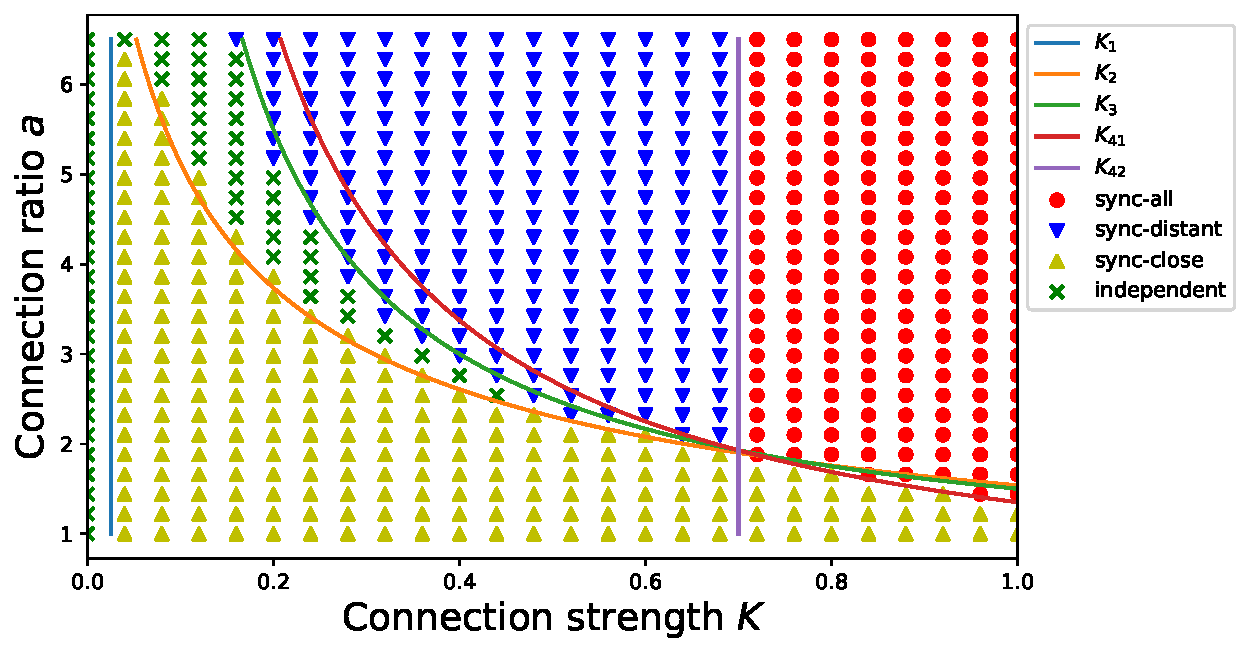
\includegraphics[width=135mm]{images/three-body-phase.pdf}
    \centering
    \caption{$\Omega=-2,\ \omega=0.05$のときの結合強度$K$,結合強度$a$における3体系の同期状態を表す分岐図.
    各格子点に対し,3体全体の同期・固有振動数の離れた振動子との同期・固有振動数の近い振動子との同期・3体とも非同期の4状態を示している.
    また,\ref{sec:3body-k12},\ \ref{sec:3body-k3},\ \ref{sec:3body-k4}節で求めた臨界結合強度の近似をそれぞれ重ねて示している.
    }
    \label{fig:3body-phase}
    \end{figure}
\section{議論}
\label{sec:3body-discussion}
\ref{sec:3body-critical}節では結合強度$K_1,\ K_2$については$|\Omega|\gg|\omega|$の場合について求めた.
また,\ref{sec:3body-summary}節では,$|\Omega|\gg|\omega|$の場合について,結合強度$K$の変化に対応する同期状態の変化パターンとその結合強度比$a$への依存性を調べた.\\
$a$を固定したときの変化パターンは,ネットワークの枝の本数を固定した場合の同期パターンに対応する.
変化パターンの$a$依存性を理解することで,既存の同期状態が分かっているネットワークに枝を追加・削除したときにどう同期状態が変化するか理解することができる.
よって,$a$を固定したときの変化パターンは枝の本数と同期状態の関係において重要な解析対象である.
したがって,他のパラメータ領域でも同様に同期状態の変化パターンの$a$依存性を調べることが期待される.\\
$|\Omega|\sim|\omega|$の場合,式\eqref{eq:3body-matome}の$K_1$は正しくない.
しかしながら,\ref{sec:3body-k3}節の議論と同様にして,固有振動数の近い振動子との同期の十分条件,つまり$K_1$の上界が与えられる.
\begin{align*}
    K_1\lessapprox\frac{|\omega|}{2-a}:=K'_1
\end{align*}
このとき,$K'_1,\ K'_3,\ K_{41},\ K_{42}$は$a^\ast_1$で一致する.
すなわち,2体が同期する場合鞍替えは起こらず,結合強度$K$を大きくしても3体の同期が起こるということになるため,これまでの議論と反する.
よって,$K'_1,\ K'_3$を用いて同期状態の変化パターンを議論するのは不適切である.
よって,一般のパラメータ領域での同期状態の変化パターンを解析する上では,$K_1,\ K_3$について$K'_1,\ K'_3$のような上界ではなくより正しい値を求めることが必要になると思われる.\\
$|\Omega|\sim|\omega|$の分岐図を図\ref{fig:3body-phase-boundary}に示す.
結合強度比$a$を大きくすると,図\ref{fig:3body-notapprox150}のような同期状態の変化パターンから,図\ref{fig:3body-notapprox175},図\ref{fig:3body-notapprox200}の順に変化パターンが変化することがわかる.
そして,3体がどれも非同期の状態から3体が同期するような図\ref{fig:3body-symmetry}のような状況は起きえないことがわかる.\\
また,他のパラメータに対し同様に数値実験を行った結果から,3体がどれも非同期の状態から3体が同期する必要十分条件が$\Omega=-\omega$であり,多くのパラメータ領域では起きえないことが推測される.
異なる振動数をもつ集団が同時に同じ振動数に変化することがほとんどのパラメータ領域では起きえないとすれば,異なる振動子の集団がほとんどの場合2つしか同時に同じ振動数に変化することはないと考えることができ,
一般のネットワークの同期状態の変化を調べるために最も簡略化された3体系に分割して解析することが正当化される.
\begin{figure}[t]
\centering
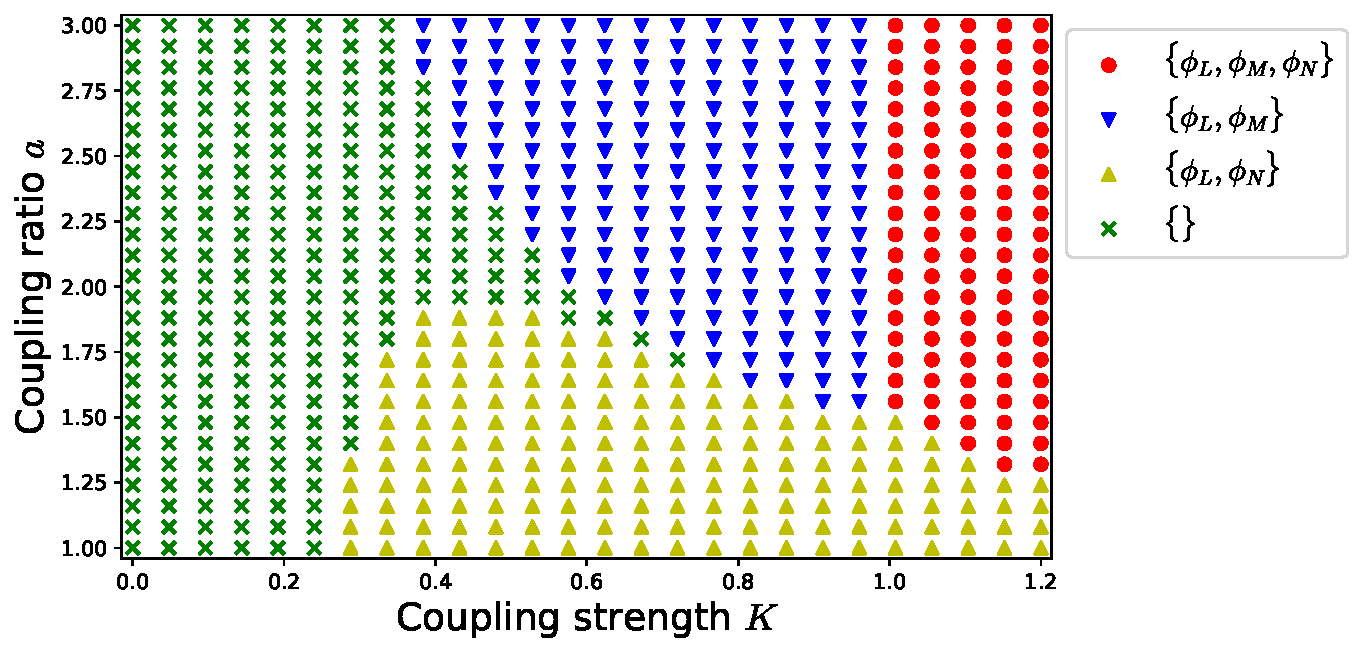
\includegraphics[width=135mm]{./images/three-body-phase-boundary.pdf}
\centering
\caption{$\Omega=-2,\ \omega=0.5$のときの結合強度$K$,結合強度$a$における3体系の同期状態を表す分岐図.
各格子点に対し,3体全体の同期・固有振動数の離れた振動子との同期・固有振動数の近い振動子との同期・3体とも非同期の4状態を示している.\\
$a=1.5,\ 1.8$を境に$a$を固定し$K$を変化させたときの同期状態の変化パターンが変化している.}
\label{fig:3body-phase-boundary}
\end{figure}
\end{document}